\documentclass[12pt]{article}
\usepackage[top=2.8cm, bottom=3cm, left=2.5cm, right=2.5cm]{geometry}
\usepackage[hidelinks]{hyperref}
\usepackage[numbers]{natbib}
\bibliographystyle{plainnat}
\usepackage{appendix}
\usepackage{caption}
\usepackage{amsmath}
\usepackage{listings}
\usepackage{setspace}
\linespread{1.2}
\lstset { %
    language=C++,
    backgroundcolor=\color{black!5}, % set backgroundcolor
    basicstyle=\ttfamily\footnotesize,% basic font setting
}
\usepackage{bchart}
\usepackage{booktabs}

\setlength{\parindent}{0em}
\setlength{\parskip}{1em}

\setlength\parindent{0pt}
\usepackage{tikz}


\title{\textbf{Parallel Computing Assignment 2 \\ Distributed Memory}}

\begin{document}
\maketitle


\tableofcontents
\listoffigures
\clearpage


\section{Approach to Parallelisation}

\subsection{Introduction}

The assignment was to implement matrix relaxation for a distributed memory architecture using MPI, on a matrix $\mathcal{M}$ of variable square dimension $d$, using $c$ MPI processes each running on its own processor on one of $n$ nodes, working to a floating point precision of $p$. Since Balena doesn't permit oversubscription, $t$ will always be $\leq c$.

My solution uses \texttt{MPI\_Scatterv} and \texttt{MPI\_Gatherv} to distribute and reassemble the matrix among processors, and \texttt{MPI\_Allreduce} to broadcast and reduce a global exit condition status each iteration.

\subsection{Partitioning the Matrix}

The primary goal in partitioning the matrix for relaxation across multiple processors was to minimise the amount of data which needs to be passed between nodes, as network I/O is orders of magnitude slower than accessing data from memory on the same node, or CPU cache.

To avoid overly complicating my solution for negligible fairness gains, I chose not to split rows of the matrix between different processes and only assigned processes a whole number of rows to work on. Relaxing a square matrix of size $n \times n$ with $c$ processes requires $(n-2)$ rows to be relaxed each iteration minus the first and last values of each row, as the array boundary values remain fixed.

Every process relaxes a minimum of $(n-2)$ div $c$ rows, where div is the integer division operation. This leaves $(n-2)$ mod $c$ cells remaining, and as MPI is SPMD and therefore not run in lockstep there is no way of predicting which processor will finish first, for the sake of simplicity this leaves the first $((n-2)$ mod $c)$ processes assigned to do $((n-2)$ div $c) + 1$ rows each.

Since each process only works on a subset of the complete matrix and there is a 1:1 ratio of MPI processes to real processors, there is no need to generate, store, or update the entire matrix on every core. This massively reduces the overhead of updating data after each iteration and the overhead of allocation.

\begin{figure}[!htbp]
        \centering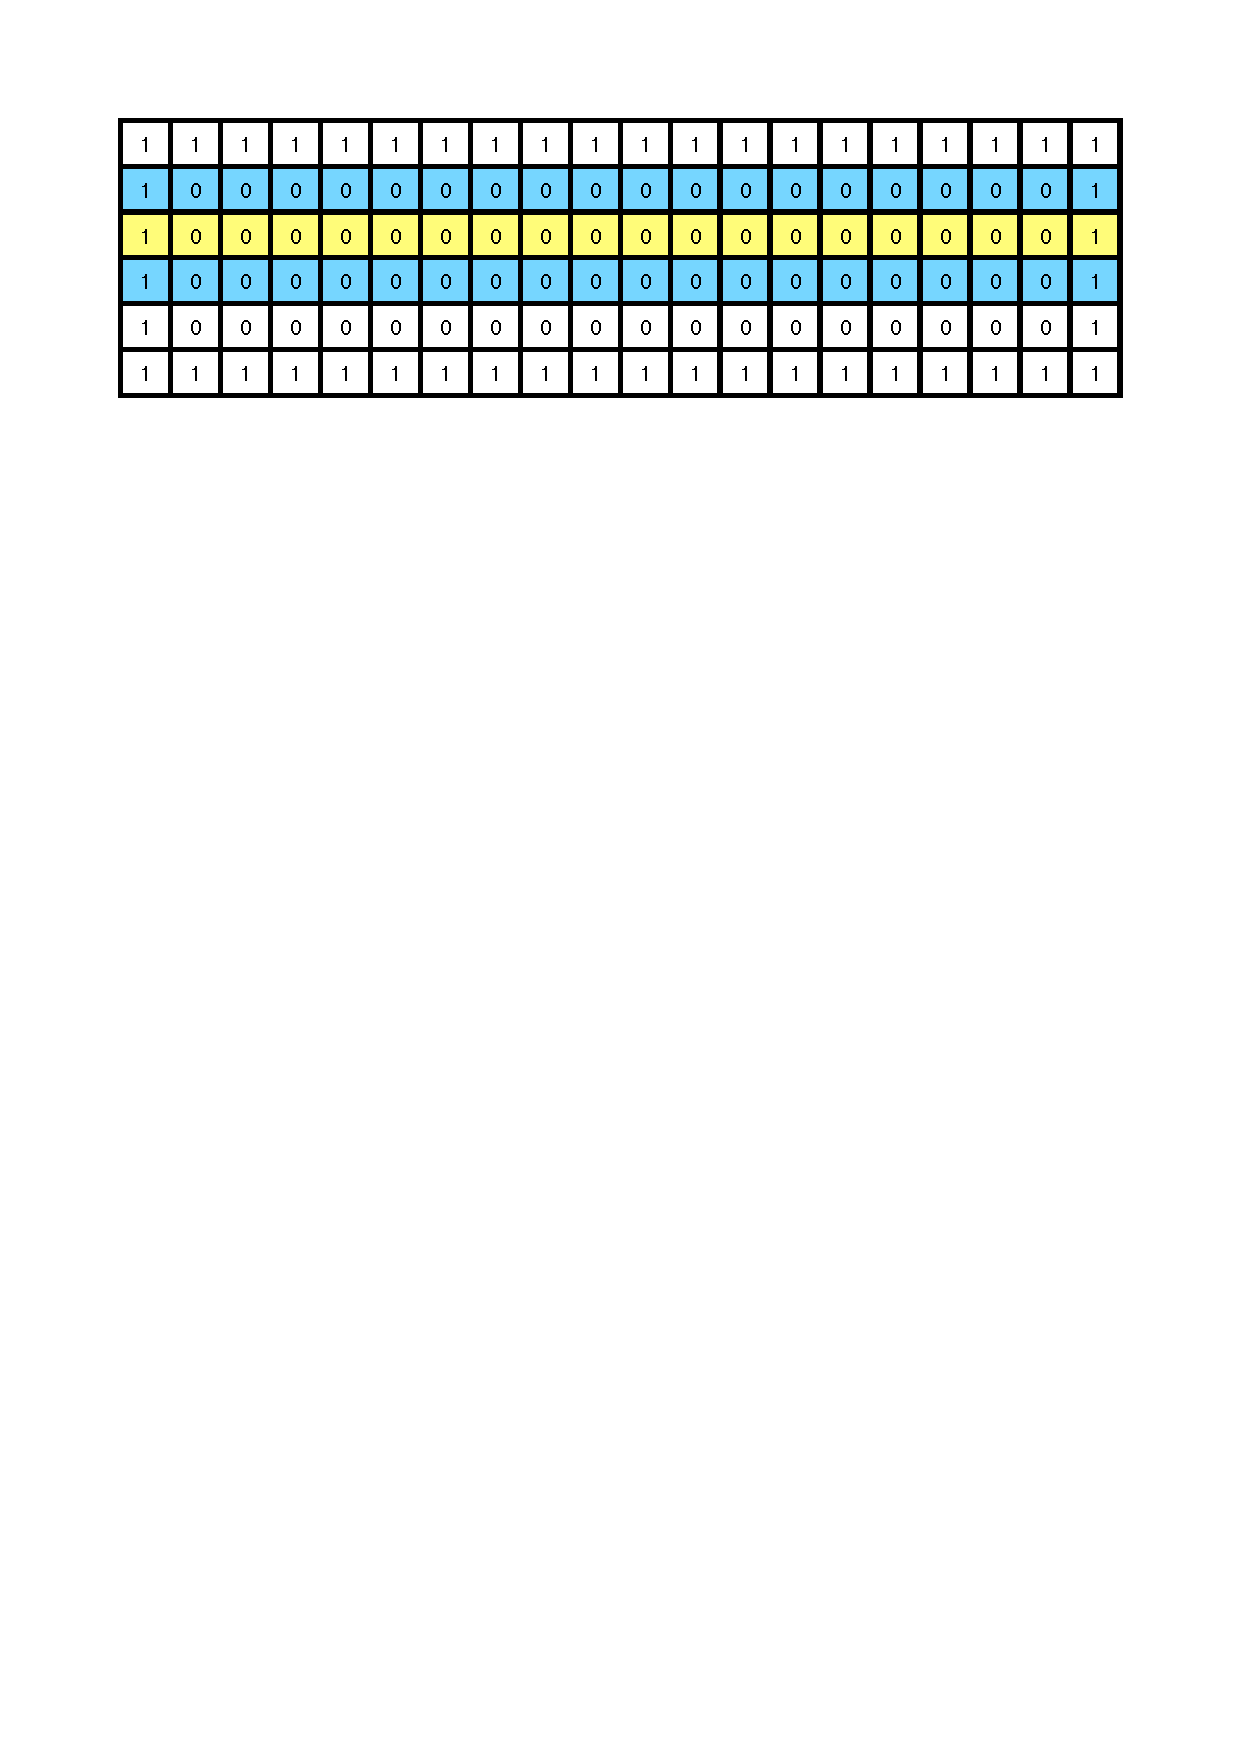
\includegraphics[width=.9\textwidth]{img/rowduplication.pdf}
        \caption{Additional rows required (blue) to relax elements in a single row (yellow).}
        \label{fig:duplicates}
    \end{figure}

As Figure \ref{fig:duplicates} illustrates, irrespective of how many partitions the matrix is split into, each CPU will require the rows immediately before and after its partition in a read-only capacity. This overhead is significant in Figure \ref{fig:duplicates} (200\%), and it can be seen that for an $n\times{n}$ matrix, it is inefficient (i.e. has an overhead $\geq$ 100\%) to have more than $\frac{n-2}{2}$ processors relaxing. From a practical parallelism standpoint, relaxing a matrix with dimensions only double that of the number of available processors is poor exploration of data parallelism and likely to be slower than a serial equivalent.

The complete $n\times{n}$ matrix is allocated and initialised from the root process and every processor (including the root) allocates space for $2n+\frac{(n-2)(n)}{c} +\frac{(n-2)(n)}{c}$ elements. The additional array of size $+\frac{(n-2)(n)}{c}$ is to preserve the consistency of data being read by performing the \textit{relax} operation; no cell can be overwritten with its new value until the new value every other cell has been calculated. This is the case regardless of whether the relaxation is performed sequentially or in parallel, and necessitates using a second matrix of the same dimensions, into which the relaxed values are written. These dimensions however, do not have to include the $2n$ read-only values from the rows above and below.

This allocation on each of $c$ processors, with an additional $n\times{n}$ on the root, gives a space complexity of $\mathcal{O}(3n^2 -4n + 2nc)$. When calculating space complexity, $c$ is constant as it is simply the number of processors so the space complexity is still asymptotic to $\mathcal{O}(n^2)$; the same space complexity as the shared memory equivalent solution which involved swapping two $n\times{n}$ arrays between iterations.

After each iteration, each process sends the $\frac{n-2}{c}$ rows which it has relaxed back to the root process. In actuality, this is not necessary because only the first and last relaxed rows contain values which are needed by any other process, so only they need to be sent. I decided not to attempt to exploit this because it introduced additional complexity, however if I were attempting to scale my solution to much larger matrices, this would be the first optimisation I would make.

An additional optimisation I could have made was in the calculation of precision. My implementation avoids iterating over cells twice by both relaxing and calculating whether the precision has been reached in the same loop, rather than calculating precision once all cells have been relaxed within a process or from the root process. However, once a process encounters a cell whose new value differs from the old by more than the specified precision, it does not have to calculate the precision for any other values. I kept calculating every value however, as some of my testing used small precision values and it was useful that the values of \texttt{local\_continue} and \texttt{global\_continue} were exactly the number of cells where precision had yet to be reached.

\subsection{MPI Strategy}

There are three types of communication which need to happen during the execution of the program, all of them every iteration:
\begin{enumerate}
	\item Sending $2+\frac{n-2}{c}$ rows of the full matrix to each process.\par
			As only a subset of the matrix is required by each process, \texttt{MPI\_Scatter} was the logical solution. However, Scatter requires all chunks to be the same size, which is only the case when $(n-2)$ mod $c=0$. The equivalent for unequal partitions is \texttt{MPI\_Scatterv}, so this is how I send data from the root process at the start of each iteration.
	
	\item Sending $\frac{n-2}{c}$ relaxed rows from each process back to the root. \par
			This communication is essentially symmetric to the previous, so I used \texttt{MPI\_Scatterv}'s counterpart \texttt{MPI\_Gatherv} to communicate the relaxed cells back to the root process.
			
	\item Communication between all processes as to whether another iteration is required.\par
			I considered adding an extra cell to each array sent back to the root process in the previous communication to piggyback the completion status of each processor with its data, but ultimately this seemed an untidy solution to a problem which \texttt{MPI\_Allreduce} could solve. I therefore reduce the \texttt{MPI\_SUM} operation over the values of \texttt{local\_continue} on every processor (where any positive value indicates a cell which has not yet reached the required precision.) If any processor needs to continue, they must all continue.
\end{enumerate}


\section{Correctness Testing}

To verify that my implementation of relaxation was correct, I manually calculated every step in relaxing a matrix and verified not only that both solutions terminated after the same number of iterations, but also that after each iteration, my matrix was identical to the computed one. Both my hand-computed relaxation (below) and my single-threaded implementation required four iterations to relax the 5$\times$5 matrix to a precision of 0.75.
\hspace{-0.2cm}\begin{minipage}{.5\textwidth}
$$
\begin{matrix}
1.000000 & 1.000000 & 1.000000 & 1.000000 & 1.000000 \\
1.000000 & 3.000000 & 7.000000 & 2.000000 & 1.000000 \\
1.000000 & 8.000000 & 6.000000 & 5.000000 & 1.000000 \\
1.000000 & 9.000000 & 0.000000 & 4.000000 & 1.000000 \\
1.000000 & 1.000000 & 1.000000 & 1.000000 & 1.000000 \\
\end{matrix}
$$
$$
\begin{matrix}
1.000000 & 1.000000 & 1.000000 & 1.000000 & 1.000000 \\
1.000000 & 4.250000 & 3.000000 & 3.500000 & 1.000000 \\
1.000000 & 4.750000 & 5.000000 & 3.250000 & 1.000000 \\
1.000000 & 2.500000 & 5.000000 & 1.750000 & 1.000000 \\
1.000000 & 1.000000 & 1.000000 & 1.000000 & 1.000000 \\
\end{matrix}
$$
$$
\begin{matrix}
1.000000 & 1.000000 & 1.000000 & 1.000000 & 1.000000 \\ 
1.000000 & 2.437500 & 3.437500 & 2.062500 & 1.000000 \\ 
1.000000 & 3.187500 & 4.000000 & 2.812500 & 1.000000 \\ 
1.000000 & 2.937500 & 2.562500 & 2.562500 & 1.000000 \\ 
1.000000 & 1.000000 & 1.000000 & 1.000000 & 1.000000 \\ 
\end{matrix}
$$
$$
\begin{matrix}
1.000000 & 1.000000 & 1.000000 & 1.000000 & 1.000000 \\ 
1.000000 & 2.156250 & 2.375000 & 2.062500 & 1.000000 \\ 
1.000000 & 2.593750 & 3.000000 & 2.406250 & 1.000000 \\ 
1.000000 & 1.937500 & 2.625000 & 1.843750 & 1.000000 \\ 
1.000000 & 1.000000 & 1.000000 & 1.000000 & 1.000000 \\ 
\end{matrix}
$$
$$
\begin{matrix}
1.000000 & 1.000000 & 1.000000 & 1.000000 & 1.000000 \\ 
1.000000 & 1.742188 & 2.054688 & 1.695312 & 1.000000 \\ 
1.000000 & 2.023438 & 2.500000 & 1.976562 & 1.000000 \\ 
1.000000 & 1.804688 & 1.945312 & 1.757812 & 1.000000 \\ 
1.000000 & 1.000000 & 1.000000 & 1.000000 & 1.000000 \\
\end{matrix}
$$
\end{minipage}\hspace{1.5cm}
\begin{minipage}{.5\textwidth}
\vspace{0.6cm}
	\textbf{Initial Matrix}\\[1.9cm]
	Max $\Delta$: $abs$(9-2.5) = 6.5\\
	6.5 $\geq$ 0.75 so continue.\\[1.6cm]
	
	Max $\Delta$: $abs$(5-2.5625) = 2.4375\\
	2.4375 $\geq$ 0.75 so continue.\\[1.6cm]
	
	Max $\Delta$: $abs$(3.4375-2.375) = 1.0625\\
	1.0625 $\geq$ 0.75 so continue.\\[1.6cm]
	
	Max $\Delta$: $abs$(2.625-1.9453125) = 0.6796875\\
	0.6796875 $<$ 0.75 (done).\\[1.9cm]
	\textbf{Relaxed matrix (after 4 iterations)}
\end{minipage}

The hand-computed results show my checking of the maximum delta for each array after relaxing it to determine whether another iteration is required. Once I verified that my implementation was correct with one thread, I relaxed under the same conditions with 2-9 threads, printing all intermediate values and the iteration count at termination. I then used the Unix \texttt{diff} utility to check all 9 outputs were identical. These files have been included in the \texttt{correctness} directory, for verification.

\section{Scalability Investigation}

\subsection{Fixed Problem Size}
Once I had verified the correctness of my relaxation implementation, I chose a fixed array size and precision, and ran my program relaxing the same array with 1-64 cores across 1-4 nodes.  The time, speedup and efficiency (speedup achieved by $n$ processors divided by $n$ \citep{speedup}) relative to the serial program can be seen in Figures \ref{fig:time15}, \ref{fig:sp15}, and \ref{fig:eff15}. 
\begin{figure}[!htbp]
        \centering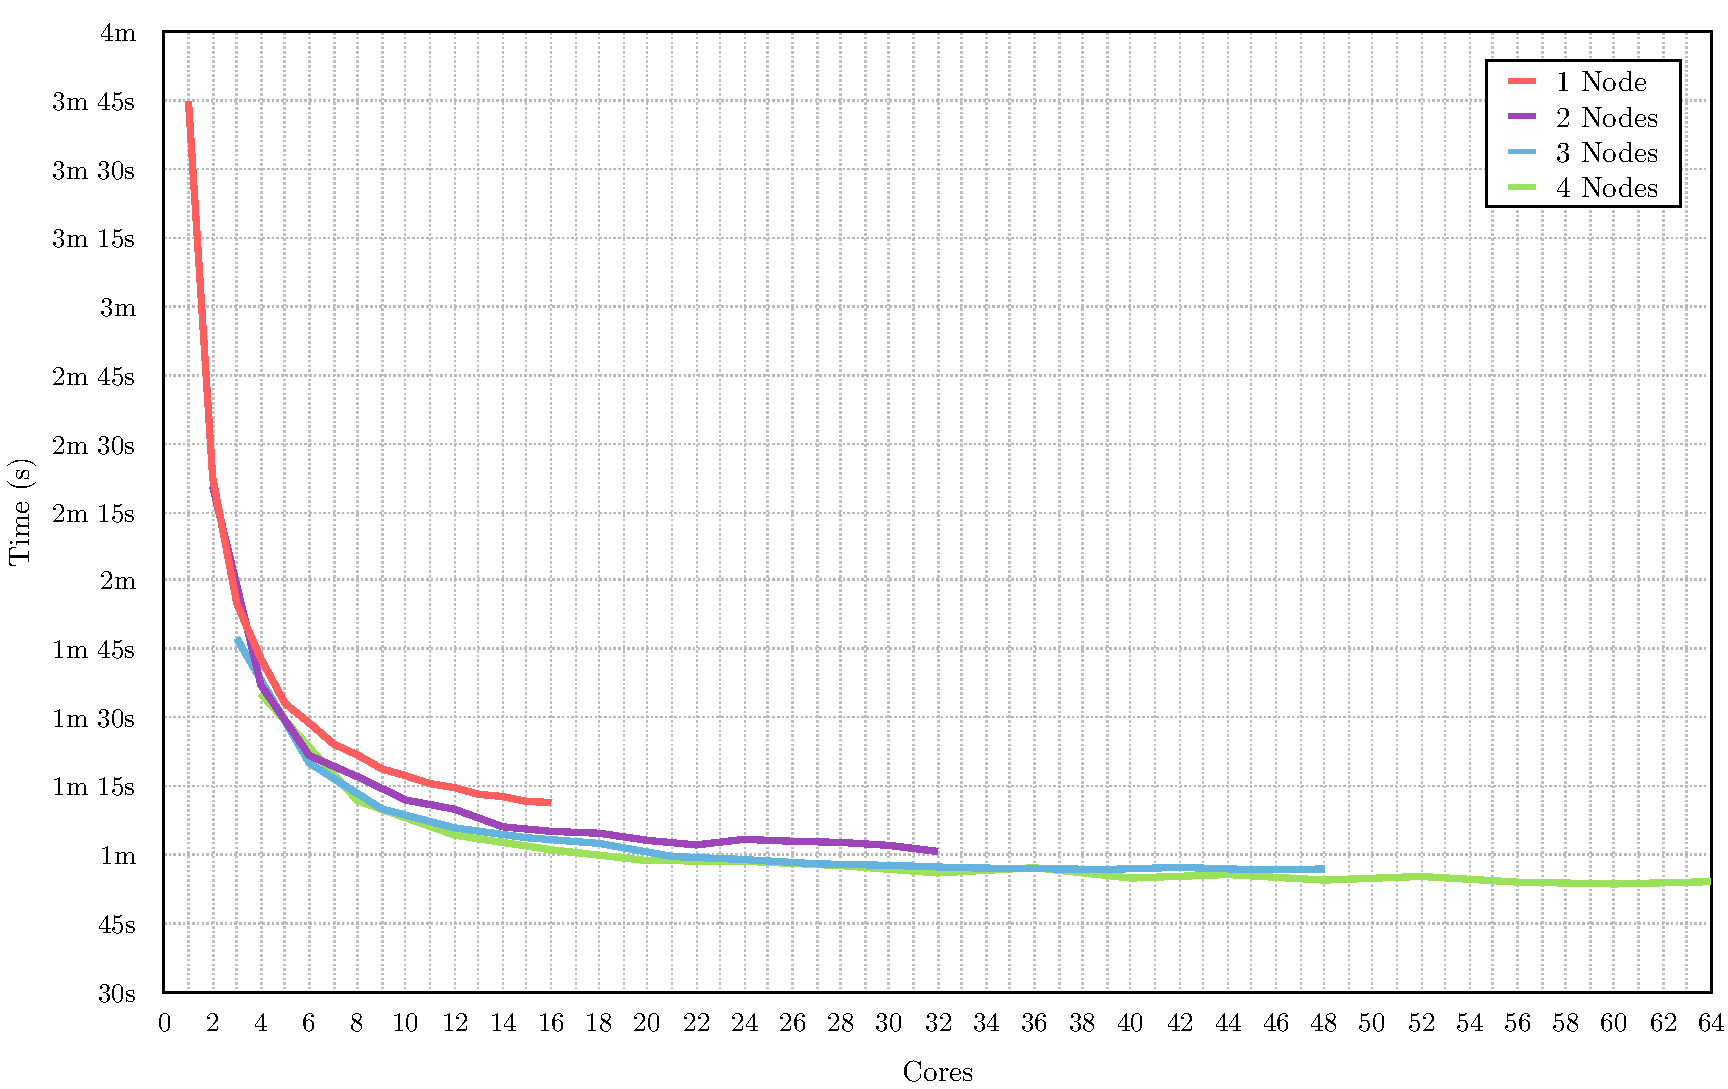
\includegraphics[width=\textwidth]{img/basic-cpus-time.pdf}
        \caption{Time taken for 1-64 cores to relax the same matrix, $d=15000$, $p=0.01$}
        \label{fig:time15}
\end{figure}
\begin{figure}[!htbp]
        \centering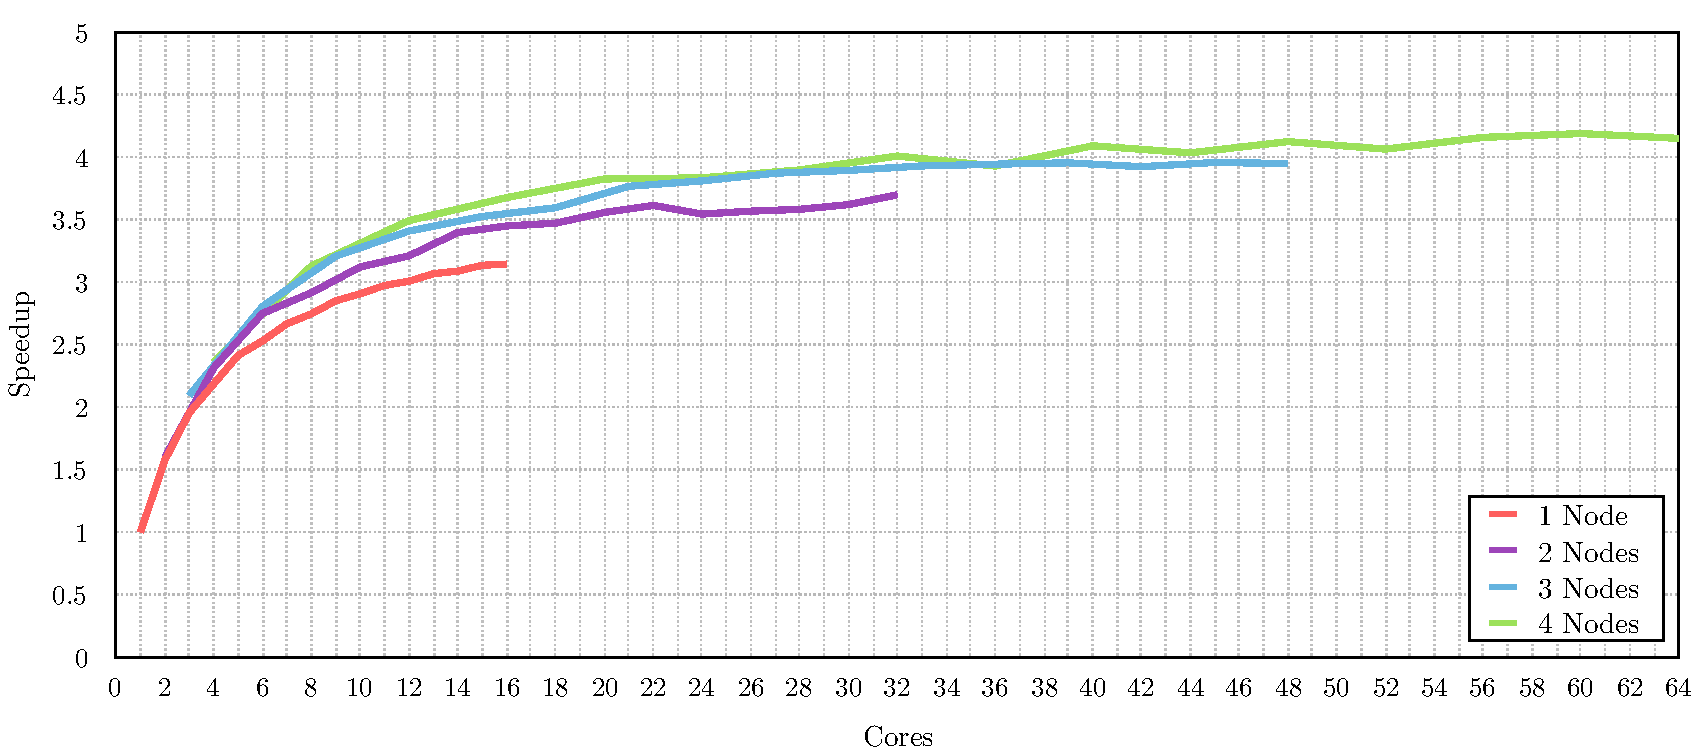
\includegraphics[width=\textwidth]{img/15kspeedup.pdf}
        \caption{Speedup achieved by 1-64 cores relaxing the same matrix, $d=15000$, $p=0.01$}
        \label{fig:sp15}
\end{figure}
\begin{figure}[!htbp]
        \centering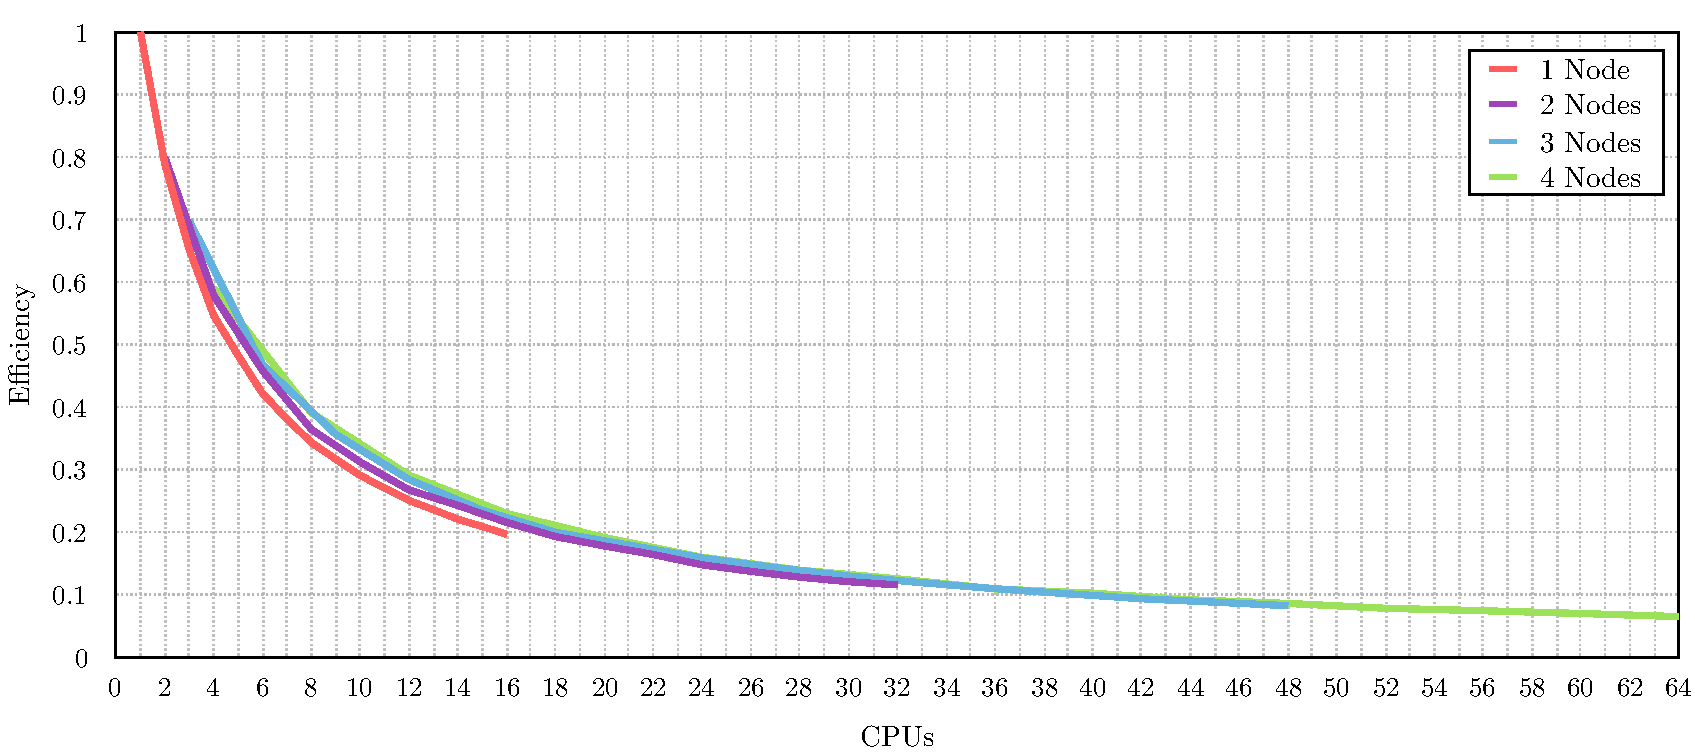
\includegraphics[width=\textwidth]{img/15kefficiency.pdf}
        \caption{Efficiency of 1-64 to relax the same matrix, $d=15000$, $p=0.01$}
        \label{fig:eff15}
\end{figure}

Each additional CPU saw efficiency reduce exponentially, as the speedup had a progressively smaller impact on the time reduction (the principle of diminishing returns; \citep{Amdahl}). This is consistent with Amdahl's law, a corollary of which states that for P processors and a computation whose sequential proportion is denoted $f$, predicted speedup is bound by $\frac{1}{f}$ \citep{springer}. Working backwards from this upper bound and assuming a maximum speedup of 4.2, this would imply that the sequential proportion of my solution is $\leq 0.238$, or 23.8\% of the total computation for this fixed problem size. It is important to note that the sequential proportion is not fixed, as changing the number of cores, precision or dimensions would alter the overhead needed to allocate, assign thread work, and wait at barriers.

Also consistent with expectation was the timing and efficiency of different configuratoins for the same number of cores; i.e. one node with 12 cores (1m 14s 745ms, 25.1\% efficiency), two nodes each with six cores (1m 10s 12ms, 26.8\% efficiency), three nodes with four cores (1m 5s 932ms, 28.4\% efficiency), and four nodes with three (1m 4s 357ms, 29.1\% efficiency). Although the absolute difference in timing between the slowest and fastest configuration is under 11 seconds, the relative efficiencies differ by 4\%. 

The speedup I achieved for this problem size was significantly sub-linear in terms of Amdahl's law. The limiting factor is the relatively slow speed of communication between cores, and as the volume of communication necessary increases proportionally to the number of cores, the overhead increases in line with this. The fact that the timing, speedup and efficiency curves are similarly asymptotic for all numbers of nodes suggests that intra-node communication speeds are not as much of a limiting factor as intra-core speeds.

\subsection{Variable Problem Size}

The second factor I tested was the effect of varying the matrix dimensions on the time, for various numbers of cores. The results of this can be seen in Figures \ref{fig:dimension-time} and \ref{fig:dimension-sp}\footnote{Full data in Appendix \ref{sec:dt}}. The x-axis in the graph is scaled according to the square of the dimensions tested rather than the dimensions themselves, as the problem size is equal to the number elements of the matrix.

\begin{figure}[htbp!]
	\centering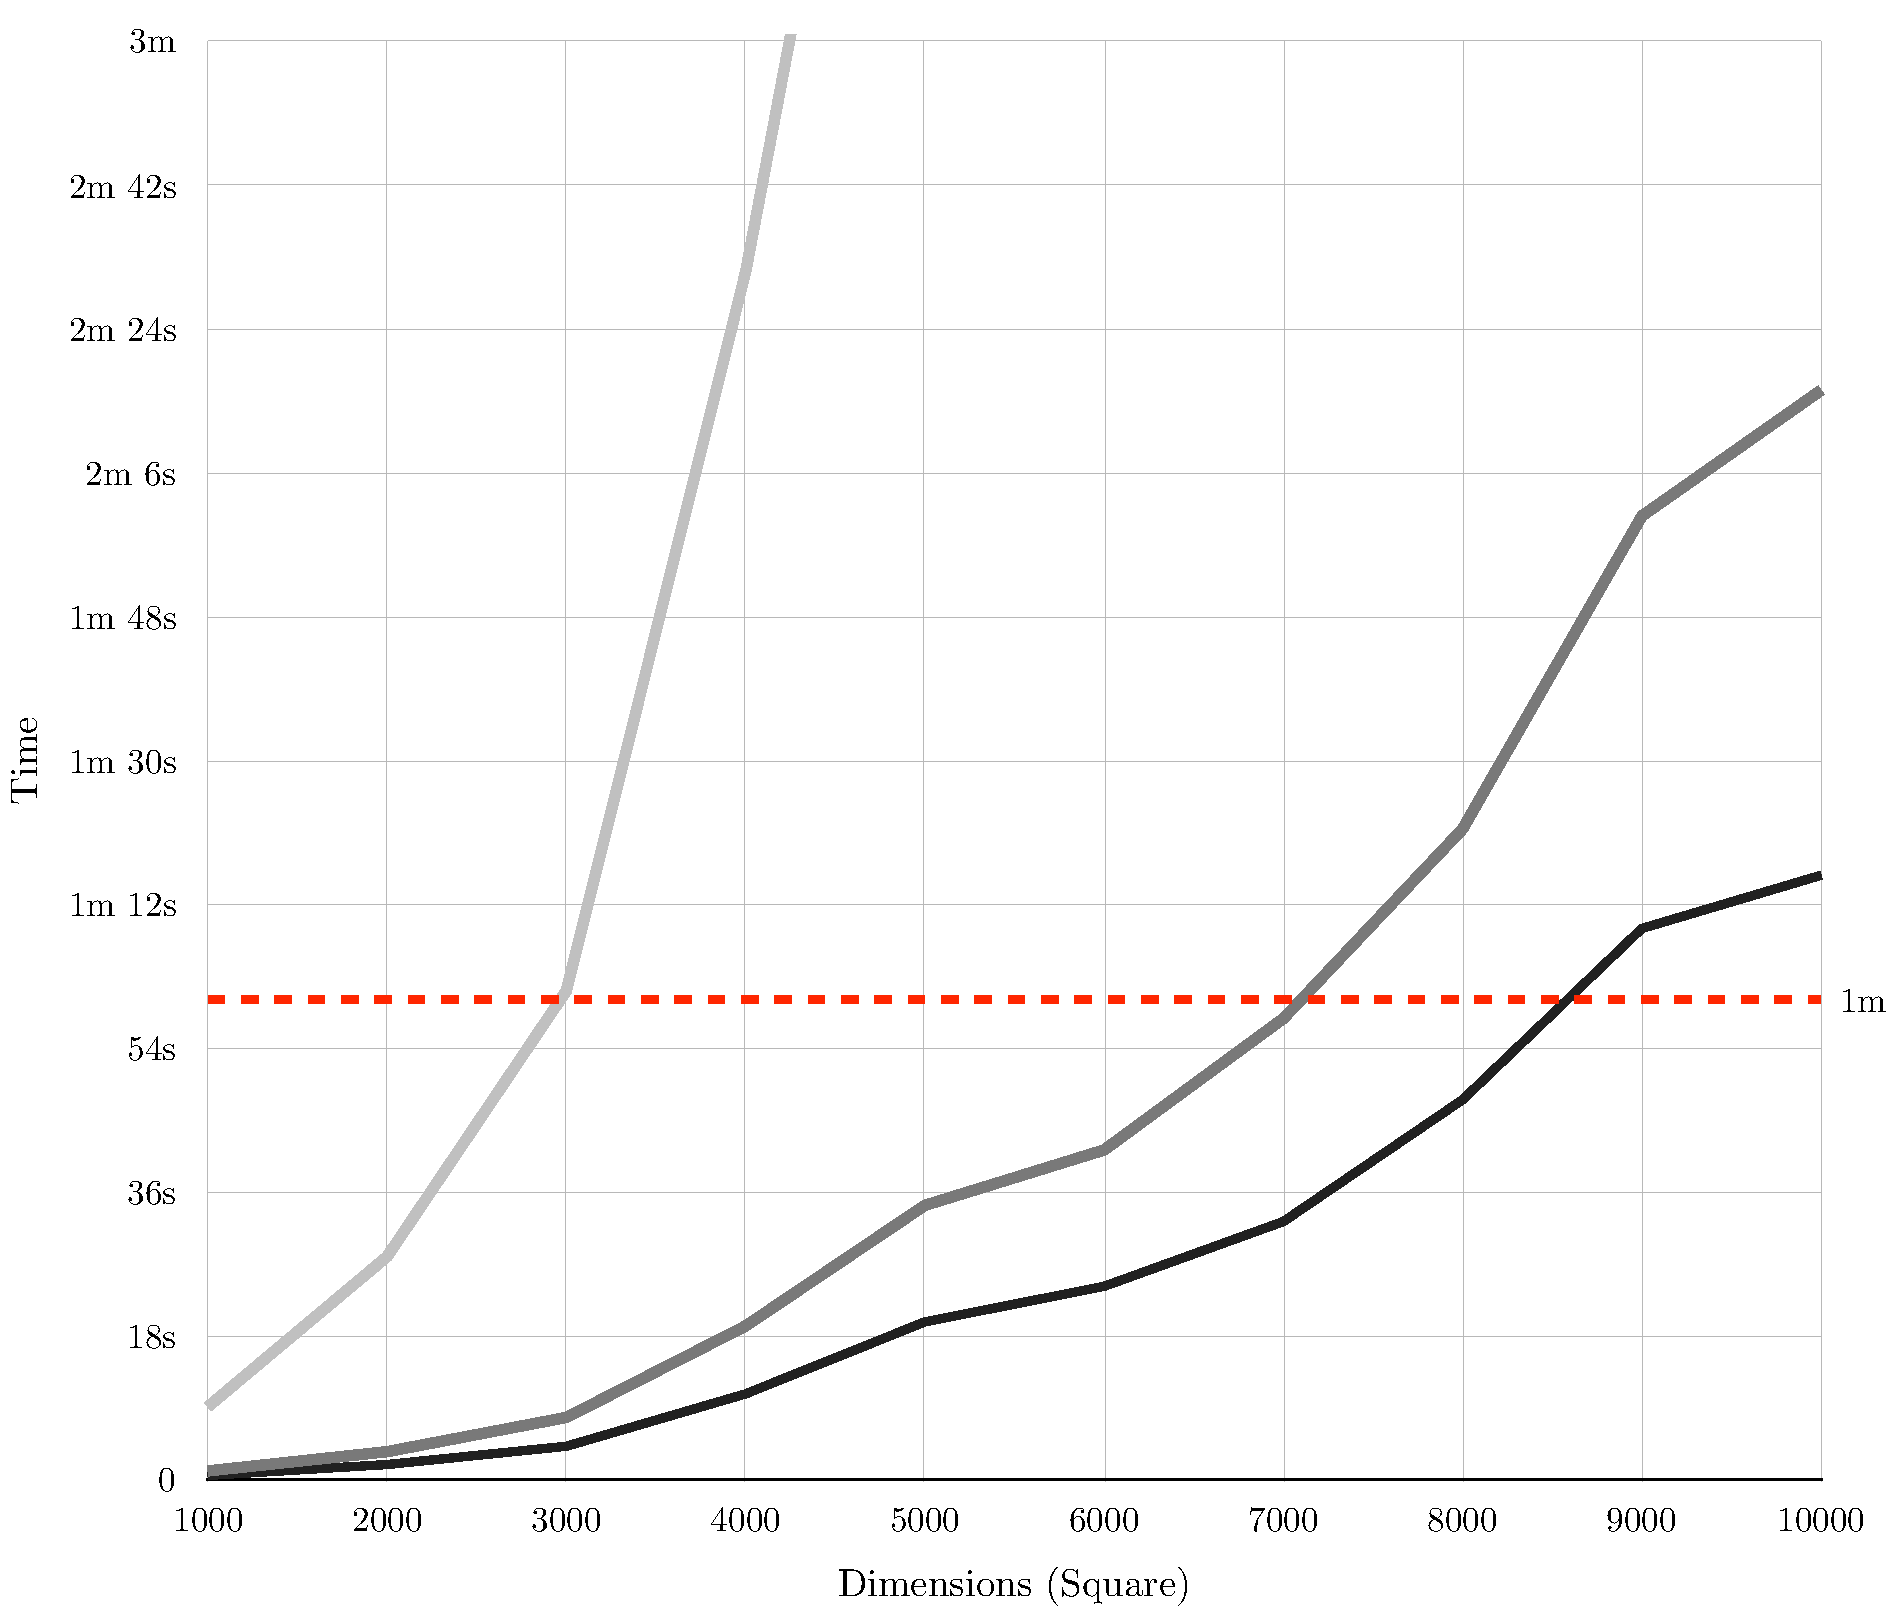
\includegraphics[width=\textwidth]{img/dimension-time.pdf}
	\caption{Matrix size against time for 16, 32, 48 and 64 cores.}
	\label{fig:dimension-time}
\end{figure}

\begin{figure}[htbp!]
	\centering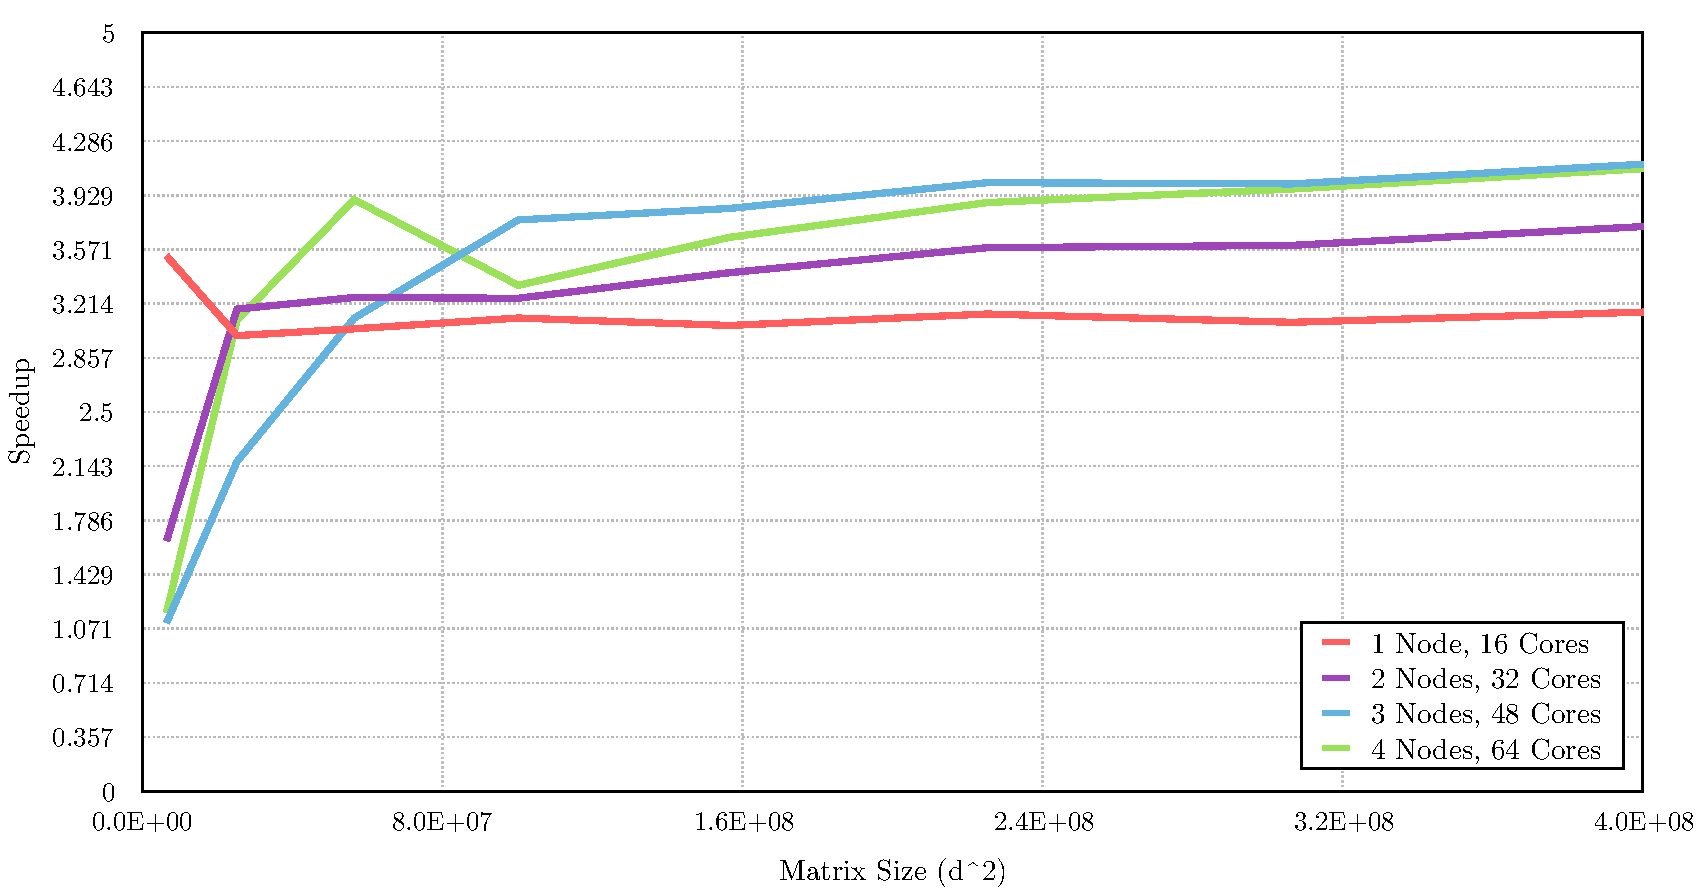
\includegraphics[width=\textwidth]{img/dimension-speedup}
	\caption{Matrix size against speedup for 16, 32, 48 and 64 cores.}
	\label{fig:dimension-sp}
\end{figure}

Time taken increases roughly linearly for a linear increase in matrix size size, as diminishing returns does not apply in the same way to variable problem sizes with fixed computational resources. The maximum matrix dimension my solutions were able to relax was $45000\times{}45000$, after which 32-64 cores exceed the ten minute timeout on Balena. Below 32 cores, the maximum dimensions reached were $42500\times{}42500$.

Figure \ref{fig:dimension-sp} shows the initial speedup achieved up until $20000\times{}20000$, at which point the serial implementation times out and there is nothing against which to benchmark speedup. Initially, 16 cores exhibits the best speedup due to the small problem size; the overhead of sending data off-core to relax dwarfs the relaxation time below $5000\times{}5000$. Above these dimensions, 16 cores settles to a stable speedup of 1.9, with 32 cores seeing an average speedup of 3.4 and 64 cores exhibiting slightly worse speedup than 48 cores above $15000\times{}15000$.

Gustafson's Law argues that as problem size increases, the sequential part of a computation decreases relatively and therefore the speedup achieved by $p$ processors for problem size $n$ is not bound by the sequential proportion $f$ as in Amdahl's law, but $p$ itself (with $S_p = p$ being perfect speedup). However, this law has been shown to be equivalent to Amdahl's law \citep{reevaluating} so I chose not to calculate speedup again.


\subsection{Precision}

I conducted a single experiment into the effects of lowering the precision threshold on the time and iterations required for my solution to terminate. Below are the results for a fixed array with $d=500$ and 16 threads\footnote{Full data in Appendix \ref{sec:prec}}, showing iterations and time increasing at the same rate as the precision threshold is lowered.

\begin{figure}[h!]
%	\hspace{-0.8cm}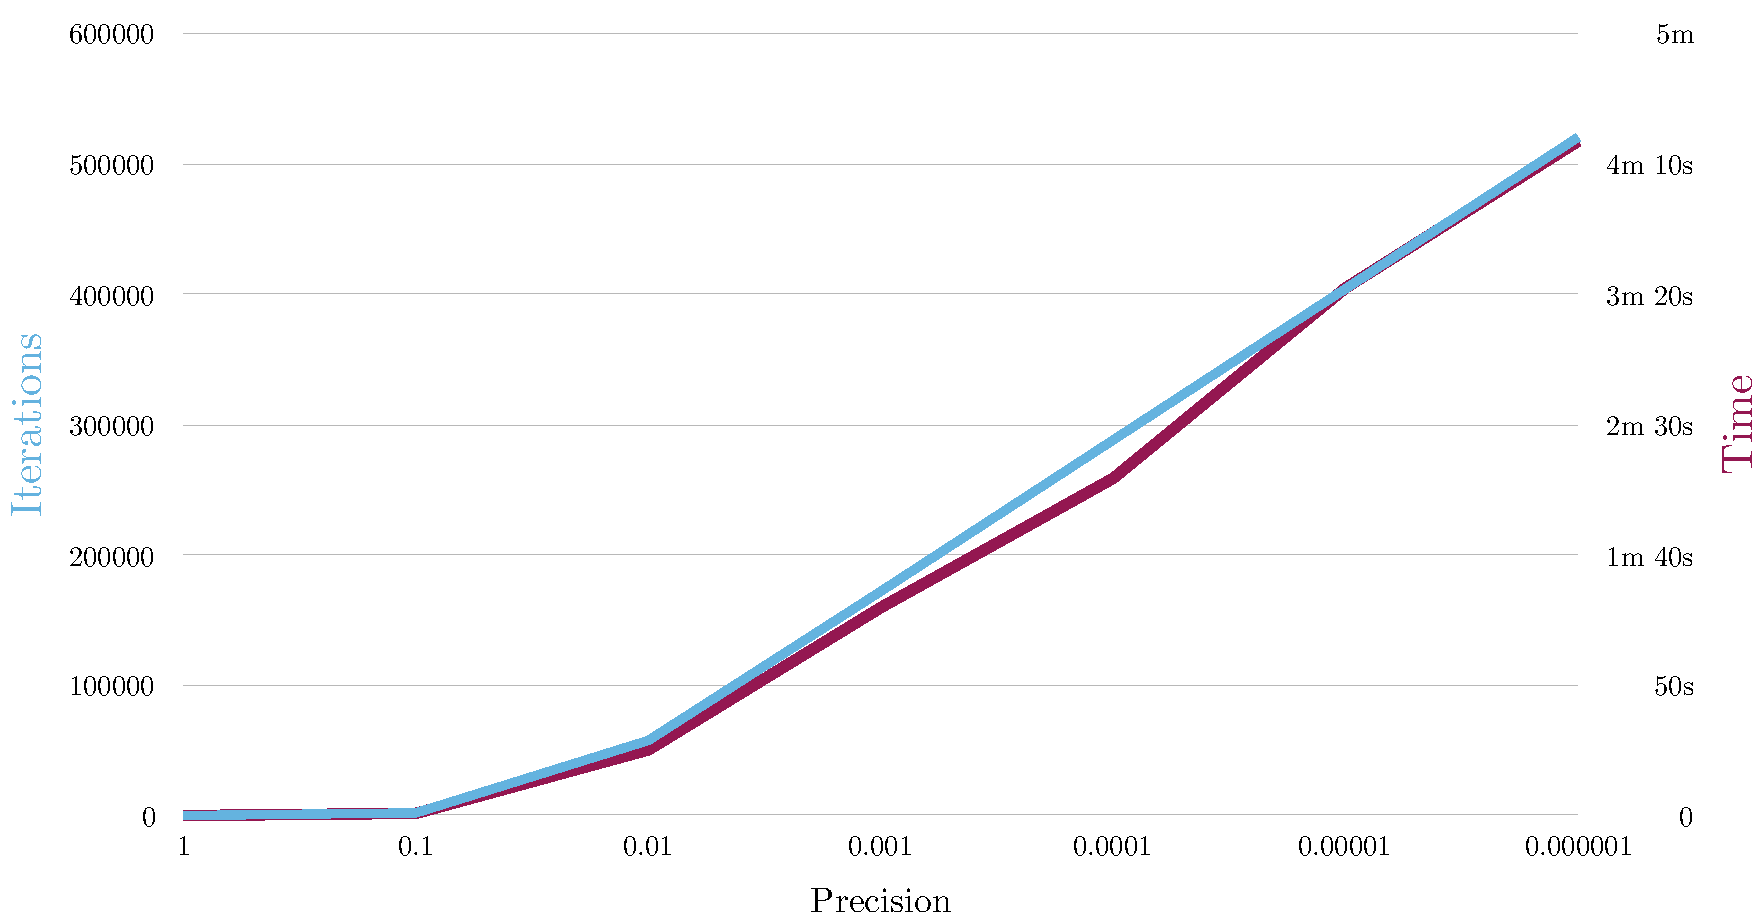
\includegraphics[width=1.1\textwidth]{img/prec-time.pdf}
	\caption{Precision values against iterations and time}
	\label{fig:precision}
\end{figure}
I tried to run my solution on a precision of 0.0000001, but it timed out on Balena, due to either exceeding the 15 minute limit while relaxing, or reaching the point at which applying the relax operation left every cell unchanged. Not every matrix when relaxed to under a given precision will terminate. My implementation does not attempt to identify these cases and would therefore loop infinitely for precision values which aren't reachable for a given matrix.

\clearpage


\bibliography{references}

\begin{appendices}

\clearpage
\section{Full Testing Results}
\subsection{Time and Speedup for 1-16 threads, $d=1000$, $p=0.5$}
\footnotesize{\label{sec:basic}
\begin{center}
\begin{tabular}{|l|l|l|}
\hline
Threads	& Time & Speedup  \\
\hline
1 & 9s 187ms & 1 \\
2 & 4s 626ms & 1.986 \\
3 & 3s 109ms & 2.955 \\
4 & 2s 343ms & 3.921 \\
5 & 1s 892ms & 4.856 \\
6 & 1s 585ms & 5.796 \\
7 & 1s 369ms & 6.711 \\
8 & 1s 205ms & 7.624 \\
9 & 1s 81ms & 8.499 \\
10 & 979ms & 9.384 \\
11 & 902ms & 10.185 \\
12 & 834ms & 11.016 \\
13 & 774ms & 11.87 \\
14 & 731ms & 12.568 \\
15 & 686ms & 13.392 \\
16 & 647ms & 14.199 \\
\hline
\end{tabular}
\end{center}}

\subsection{Time and Speedup for 2-32 threads, $d=1000$, $p=0.5$}
\footnotesize{\label{sec:cliff}
\begin{center}
\begin{tabular}{|l|l|l|}
\hline
Threads	& Time & Speedup  \\
\hline
2 & 4s 624ms & 1.987 \\
4 & 2s 342ms & 3.923 \\
6 & 1s 591ms & 5.774 \\
8 & 1s 214ms & 7.568 \\
10 & 982ms & 9.355 \\
12 & 833ms & 11.029 \\
14 & 726ms & 12.654 \\
16 & 653ms & 14.069 \\
18 & 1s 103ms & 8.329 \\
20 & 1s 60ms & 8.667 \\
22 & 1s 126ms & 8.159 \\
24 & 1s 129ms & 8.137 \\
26 & 1s 103ms & 8.329 \\
28 & 1s 71ms & 8.578 \\
30 & 1s 53ms & 8.725 \\
32 & 1s 30ms & 8.919 \\
\hline
\end{tabular}
\end{center}}

\subsection{Dimensions against time, $p=0.5$, $t=\{1, 8, 16\}$}
\footnotesize{\label{sec:dt}
\begin{center}
\begin{tabular}{|l|l|l|l|}
\hline
Dimension & 1 Thread & 8 Threads & 16 Threads \\
\hline
1000 & 9s 231ms & 1s 207ms & 646ms \\
2000 & 28s 13ms & 3s 616ms & 2s 7ms \\
3000 & 1m 1s 257ms & 7s 896ms & 4s 291ms \\
4000 & 2m 31s 143ms & 19s 331ms & 10s 843ms \\
5000 & 4m 29s 167ms & 34s 413ms & 19s 845ms \\
6000 & 5m 23s 100ms & 41s 339ms & 24s 290ms \\
7000 & 7m 29s 558ms & 57s 778ms & 32s 389ms \\
8000 & (timed out) & 1m 21s 480ms & 47s 624ms \\
9000 & (timed out) & 2m 0s 608ms & 1m 9s 36ms \\
10000 & (timed out) & 2m 16s 340ms & 1m 15s 692ms \\
\hline
\end{tabular}
\end{center}}

\subsection{Precision against iterations and time, $d=500$, $t=16$}
\footnotesize{\label{sec:prec}
\begin{center}
\begin{tabular}{|l|l|l|}
\hline
Precision	& Time & Iterations  \\
\hline
1 & 38ms & 78 \\
0.1 & 872ms & 2160 \\
0.01 & 25s 239ms & 57755 \\
0.001 & 1m 19s 879ms & 172235 \\
0.0001 & 2m 9s 480ms & 288416 \\
0.00001 & 3m 22s 586ms & 404599 \\
0.000001 & 4m 18s 886ms & 520783 \\
0.0000001 & (timed out) & (timed out) \\
\hline
\end{tabular}
\end{center}}

	
\end{appendices}

\end{document}